% The Clever Algorithms Project: http://www.CleverAlgorithms.com
% (c) Copyright 2011 Jason Brownlee. Some Rights Reserved. 
% This work is licensed under a Creative Commons Attribution-Noncommercial-Share Alike 2.5 Australia License.

% Name
% The algorithm name defines the canonical name used to refer to the technique, in addition to common aliases, abbreviations, and acronyms. The name is used in terms of the heading and sub-headings of an algorithm description.
\section{LASSO} 
\label{sec:lasso}
\index{LASSO}
\index{Least Absolute Shrinkage and Selection Operator}

% other names
% What is the canonical name and common aliases for a technique?
% What are the common abbreviations and acronyms for a technique?
\emph{LASSO, Lasso, Least Absolute Shrinkage and Selection Operator}

% Taxonomy: Lineage and locality
% The algorithm taxonomy defines where a techniques fits into the field, both the specific subfields of Computational Intelligence and Biologically Inspired Computation as well as the broader field of Artificial Intelligence. The taxonomy also provides a context for determining the relation- ships between algorithms. The taxonomy may be described in terms of a series of relationship statements or pictorially as a venn diagram or a graph with hierarchical structure.
\subsection{Taxonomy}
% To what fields of study does a technique belong?
LASSO is a Regularization method for Multiple Linear Regression models.
% What are the closely related approaches to a technique?
LASSO is related to other Regularized Regression models such as Ridge Regression.
% extensions
Least Angle Regression (LARS) is an alternate solution to the LASSO.
Group LASSO and Elastic Net are extensions of the LASSO.


% Strategy: Problem solving plan
% The strategy is an abstract description of the computational model. The strategy describes the information processing actions a technique shall take in order to achieve an objective. The strategy provides a logical separation between a computational realization (procedure) and a analogous system (metaphor). A given problem solving strategy may be realized as one of a number specific algorithms or problem solving systems. The strategy description is textual using information processing and algorithmic terminology.
\subsection{Strategy}
% What is the information processing objective of a technique?
The information processing objective of the LASSO is to reduce or shrink the magnitude of the coefficients in a regression model (called an $L_1$-penalty).
% What is a techniques plan of action?
This is achieved by penalising models based on the sum of the absolute value of the coefficients being less than a constant parameter ($t$). This constraint both shrinks the value of coefficients and allows some coefficients to be come exactly zero (unlike Ridge Regression). The effect is that this modification of least squares regression performs both continuous shrinkage of coefficients and automatic selection of variables simultaneously. The LASSO equation may be described as a quadratic programming problem with linear inequality constraints, where $t$ controls the amount of shrinkage applied to the coefficients.

% Heuristics: Usage guidelines
% The heuristics element describe the commonsense, best practice, and demonstrated rules for applying and configuring a parameterized algorithm. The heuristics relate to the technical details of the techniques procedure and data structures for general classes of application (neither specific implementations not specific problem instances). The heuristics are described textually, such as a series of guidelines in a bullet-point structure.
\subsection{Heuristics}
% What are the suggested configurations for a technique?
% What are the guidelines for the application of a technique to a problem instance?

\begin{itemize}
	\item It has been shown to achieve some of the benefits of both Subset Selection (feature selection) and Ridge Regression (shrinkage of coefficients).
	\item The penalisation scheme is general and can be applied to models beyond regression.
	\item The sparse model representation (feature) achieved by the LASSO can lead simpler models that are easier to interpret. 
	\item It is most suited for datasets where there are are a large number of small effects and least suited to problems where there are a small number of large effects.  
	\item Zou and Hastie describe three limitations of the LASSO: a) in $p>n$ problems (more variables than observations) the LASSO is limited to selecting $n$ variables, b) it selects one variable from the group of variables that pairwise highly-correlated, c) it is outperformed by ridge regression when there is high correlation between variables \cite{Zou2005}.
\end{itemize}

% sample script in R
\subsection{Code Listing}
% listing
Listing~\ref{lars_lasso_regression} provides a code listing of the LASSO method in R.
% algorithm and package
The example uses the \texttt{lars()} function in the \texttt{lars} core package. The \texttt{lars} package provides the Least Angle Regression, Lasso, and the Forward Stagewise algorithms for regularization \cite{Hastie2011}. Figure~\ref{plot:lasso_result} provides a plot of the final coefficient values of each model for the given lambda values. For more information on this library type: \texttt{library(help="lars")}, and for more information on the function type: \texttt{?lars}.

% problem
The test problem is a four-dimensional dataset of 100 samples, where \texttt{x3} and \texttt{y} are dependent on \texttt{x1} and \texttt{x1} and \texttt{x2} are independent variables. The problem is ill defined as \texttt{y} given \texttt{x1, x2, x3}. The model is expected to reduce the contribution of \texttt{x2} and \texttt{x3} toward zero leaving \texttt{y} given \texttt{x1}.

% TODO provide a better problem with real variable selection

\lstinputlisting[firstline=7,language=r,caption={Example of LASSO in R using the \texttt{lars()} function in the \texttt{lars} package.}, label=lars_lasso_regression]{../src/algorithms/regularization/lars_lasso_regression.R}

\begin{figure}[htp]
\centering
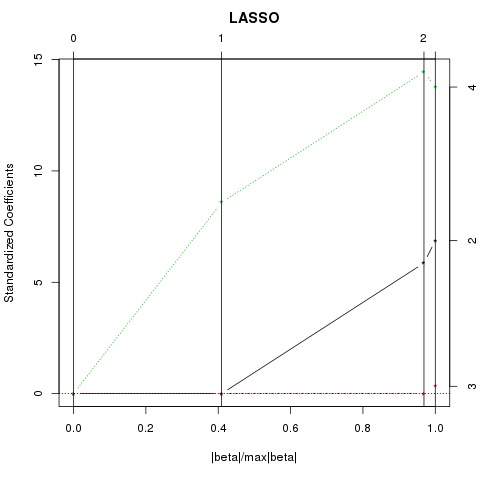
\includegraphics[scale=0.60]{a_regularization/lasso_result.png}
\caption{XXX.}
\label{plot:lasso_result}
\end{figure}

% other packages
Other packages provide implementations of the Lasso penalty method.
The \texttt{glmnet} package provides the Lasso and elastic-net regularization for generalized linear models \cite{Friedman2011}.
The \texttt{grplasso} package provides an the Group Lasso penalty method for fitting models \cite{Meier2009}.
The \texttt{grpreg} package provides lasso regularization with grouped covariates \cite{Brehen2011}.

% lmmlasso package?!?
% penalized package

% References: Deeper understanding
% The references element description includes a listing of both primary sources of information about the technique as well as useful introductory sources for novices to gain a deeper understanding of the theory and application of the technique. The description consists of hand-selected reference material including books, peer reviewed conference papers, journal articles, and potentially websites. A bullet-pointed structure is suggested.
\subsection{References}
% What are the primary sources for a technique?
% What are the suggested reference sources for learning more about a technique?

% primary sources
\subsubsection{Primary Sources}
% primary
The LASSO was described in detail by Tibshirani who also provided a Bayes model for the LASSO, simulation studies and extensions to generalization regression and other problems \cite{Tibshirani1996}. Tibshirani attributes the motivation the LASSO to Breiman's Non-negative Garrotte regression method \cite{Breiman1993} (later published \cite{Breiman1995}).

% more info
\subsubsection{More Information}
Fu provides an in depth study comparing the LASSO to Bridge Regression \cite{Fu1998}.
% extensions
Efron et~al.\ describe Least Angle Regression (LARS) which can solve the LASSO \cite{Efron2002}.
Zou and Hastie describe the Elastic Net which combines the LASSO with LARS \cite{}.

% END
